% !TEX root = ../thesis.tex

\chapter{Analýza požiadaviek}\label{ch:requirements-analysis}

Analýza požiadaviek sa zameriava na identifikáciu kľúčových oblastí navrhovaného informačného systému pre správu distribúcie vody, evidenciu revízií a servisných zásahov. Cieľom analýzy je previesť počiatočné textové požiadavky do formálnejšej podoby, ktorá bude použiteľná pri návrhu architektúry, databázového modelu a používateľských scenárov.

Výsledkom tejto fázy je systematické rozdelenie požiadaviek do štruktúrovaných kategórií, určenie ich priority a prepojenie na zdroje. Takto spracované požiadavky vytvárajú jednotný podklad pre implementáciu, testovanie a následné vyhodnotenie riešenia.

\section{Štruktúrovaná tabuľková reprezentácia požiadaviek}

Pri návrhu systému je dôležité, aby boli požiadavky definované jednoznačne, porovnateľne a overiteľne. Tabuľková reprezentácia umožňuje každú požiadavku presne identifikovať a priradiť jej vlastnosti, ktoré podporujú rozhodovanie o rozsahu implementácie.

V tejto kapitole je každá požiadavka opísaná prostredníctvom nasledujúcich atribútov:

\begin{itemize}
\item \textbf{ID}: jednoznačný identifikátor požiadavky.
\item \textbf{Popis požiadavky}: stručná formulácia očakávanej funkcionality.
\item \textbf{Klasifikácia}: zaradenie požiadavky do vecnej oblasti systému.
\item \textbf{Priorita}: dôležitosť požiadavky pre základnú prevádzku a implementačné poradie.
\item \textbf{Zdroj}: označenie pôvodu požiadavky (UR/SR) podľa jej charakteru.
\end{itemize}

Tabuľka \ref{tab:functional-requirements-structured} prezentuje funkčné požiadavky identifikované v predchádzajúcej kapitole. Tabuľka \ref{tab:nonfunctional-requirements-structured} dopĺňa ich nefunkčné požiadavky.

\subsection{Funkčné požiadavky}

\small
\begin{longtable}{|p{1.3cm}|p{5.8cm}|p{2.0cm}|c|p{2.1cm}|}
\caption{Štruktúrovaná tabuľková reprezentácia funkčných požiadaviek}\label{tab:functional-requirements-structured}\\
\hline
ID & Popis požiadavky & Klasifikácia & Priorita & Zdroj \\
\hline
\endfirsthead
\hline
ID & Popis požiadavky & Klasifikácia & Priorita & Zdroj \\
\hline
\endhead
FR-01 & Založenie karty zariadenia s identifikátorom, typom, umiestnením, stavom a dátumom uvedenia do prevádzky. & \shortstack[l]{Evidencia\\zariadení} & 5 & UR \\
\hline
FR-02 & Úprava údajov zariadenia s evidenciou histórie zmien. & \shortstack[l]{Evidencia\\zariadení} & 5 & UR \\
\hline
FR-03 & Vyhľadávanie a filtrovanie zariadení podľa typu, lokality, stavu a zodpovednej osoby. & \shortstack[l]{Evidencia\\zariadení} & 4 & UR \\
\hline
FR-04 & Plánovanie revízie zariadenia s termínom, rozsahom a pridelenou zodpovednou osobou. & Revízie & 5 & SR \\
\hline
FR-05 & Záznam výsledku revízie vrátane stavu, poznámky a príloh. & Revízie & 5 & SR \\
\hline
FR-06 & Zobrazenie histórie revízií zariadenia v časovom poradí. & Revízie & 4 & SR \\
\hline
FR-07 & Založenie servisného zásahu na základe poruchy, revízie alebo manuálne. & Servis & 5 & UR \\
\hline
FR-08 & Evidencia priebehu servisného zásahu vrátane vykonaných prác, použitého materiálu a zodpovednej osoby. & Servis & 4 & UR \\
\hline
FR-09 & Automatické odoslanie notifikácie pred plánovaným termínom revízie. & Notifikácie & 4 & SR \\
\hline
FR-10 & Automatické odoslanie notifikácie pri prekročení termínu revízie alebo servisného zásahu. & Notifikácie & 4 & SR \\
\hline
FR-11 & Generovanie reportu revízií za zvolené obdobie. & Reporty & 4 & UR \\
\hline
FR-12 & Export reportov minimálne do formátov PDF a CSV. & Reporty & 3 & SR \\
\hline
\end{longtable}

\subsection{Nefunkčné požiadavky}

\small
\begin{longtable}{|p{1.5cm}|p{5.8cm}|p{2.0cm}|c|p{2.1cm}|}
\caption{Štruktúrovaná tabuľková reprezentácia nefunkčných požiadaviek}\label{tab:nonfunctional-requirements-structured}\\
\hline
ID & Popis požiadavky & Klasifikácia & Priorita & Zdroj \\
\hline
\endfirsthead
\hline
ID & Popis požiadavky & Klasifikácia & Priorita & Zdroj \\
\hline
\endhead
NFR-01 & Systém musí vyžadovať autentifikáciu používateľa a autorizáciu prístupu podľa pridelenej roly. & Bezpečnosť & 5 & SR \\
\hline
NFR-02 & Systém musí zabezpečiť šifrovaný prenos dát medzi klientom a serverom pomocou protokolu HTTPS. & Bezpečnosť & 5 & SR \\
\hline
NFR-03 & Systém musí zaznamenávať dôležité operácie používateľov do auditného záznamu. & Bezpečnosť & 4 & SR \\
\hline
NFR-04 & Systém musí poskytovať responzívne webové rozhranie použiteľné na desktopových aj mobilných zariadeniach. & Použiteľnosť & 4 & UR \\
\hline
NFR-05 & Systém musí poskytovať stabilnú prevádzku pri bežnej súbežnej práci viacerých používateľov bez straty dát. & Dostupnosť & 4 & SR \\
\hline
NFR-06 & Systém musí podporovať pravidelné zálohovanie dát a obnovu po zlyhaní. & Spoľahlivosť & 4 & SR \\
\hline
NFR-07 & Systém musí umožniť export dát v štandardných formátoch pre použitie v ďalších nástrojoch organizácie. & Integrácia & 3 & SR \\
\hline
NFR-08 & Systém musí byť navrhnutý modulárne, aby bolo možné jednoducho rozširovať funkcionalitu o nové moduly. & Rozšíriteľnosť & 3 & UR \\
\hline
\end{longtable}

\noindent
Priorita je hodnotená na škále 1 až 5, kde 5 predstavuje kritickú požiadavku pre základnú prevádzku systému a 1 predstavuje požiadavku s najnižšou implementačnou prioritou.

\noindent
Označenia zdrojov: \textbf{UR} (User Requirements) a \textbf{SR} (System Requirements) vyjadrujú charakter požiadavky. \textbf{UR} predstavuje požiadavky odvodené z používateľských potrieb a prevádzkových procesov, kým \textbf{SR} predstavuje systémové požiadavky odvodené z legislatívnych a odborných podkladov, najmä \cite{EUDWD2020,SKVyhlaska912023,CarricoFerreira2021}.

\section{Aktéri a okolie systému}
\label{sec:akteri-okolie-systemu}

Navrhovaný informačný systém (ďalej len ``IS'') podporuje správu distribúcie pitnej a úžitkovej vody so zameraním na evidenciu filtračných zariadení a riadenie ich revízií (plánovanie, vykonanie, protokoly, nápravné opatrenia). Z hľadiska analýzy požiadaviek je kľúčové určiť (1) aktérov, ktorí so systémom priamo pracujú alebo z neho čerpajú výstupy, a (2) okolie systému (externé systémy a služby), s ktorými IS typicky komunikuje.

Keďže medzi nefunkčné požiadavky patrí autentifikácia a autorizácia podľa pridelenej roly (NFR-01), prístupové práva sú definované pomocou modelu RBAC (Role-Based Access Control), t. j. oprávnenia sú priradené rolám a používatelia získavajú oprávnenia aktiváciou svojej roly \cite{NISTRBACGlossary,NISTRBACProject}.

\subsection{Interní aktéri systému}

Interní aktéri (roly) predstavujú používateľov, ktorí vykonávajú operatívne činnosti v systéme a priamo vytvárajú alebo spravujú artefakty identifikované v Kapitole~5 (zariadenie, filtračné zariadenie, revízia, servisný zásah, notifikácia, report, používateľ).
Prehľad rolí a ich zodpovedností je uvedený v~\autoref{tab:internal-actors}.

\begin{table}[!htbp]
\centering
\small
\renewcommand{\arraystretch}{1.2}
\begin{tabular}{p{34mm} p{110mm}}
\toprule
\textbf{Rola} & \textbf{Hlavné zodpovednosti a typické činnosti v IS} \\
\midrule
Administrátor systému (ADM) & Správa používateľských účtov a rolí, konfigurácia oprávnení (RBAC), nastavenie integračných parametrov, dohľad nad auditnými záznamami, prevádzková konfigurácia (notifikácie, exporty, pravidlá). \\
\midrule
Správca siete / prevádzky (NET) & Evidencia a aktualizácia registra zariadení (vrátane väzieb), plánovanie revízií a priraďovanie zodpovedných osôb, koordinácia servisných zásahov, kontrola plnenia termínov, správa prevádzkových prehľadov. \\
\midrule
Technik údržby (TECH) & Realizácia servisných zásahov (plánovaných aj ad-hoc), dopĺňanie záznamov o opravách, použitom materiáli a trvaní práce, aktualizácia stavu zariadenia po zásahu, reakcia na notifikácie o poruche alebo incidente. \\
\midrule
Revízny pracovník (REV) & Vykonávanie revízií filtračných zariadení podľa harmonogramu a legislatívnych požiadaviek, vyplnenie revízneho záznamu, priloženie protokolov/fotodokumentácie, zaznamenanie nedostatkov a návrh nápravných opatrení. \\
\midrule
Manažér / vedúci prevádzky (MAN) & Manažérsky dohľad nad plnením revíznych termínov a stavom zariadení, generovanie súhrnných reportov pre riadenie a audit, vyhodnocovanie trendov (poruchovosť, náklady, oneskorenia), kontrola súladu procesov. \\
\bottomrule
\end{tabular}
\caption{Interní aktéri systému a ich hlavné zodpovednosti.}
\label{tab:internal-actors}
\end{table}

\subsection{Externí aktéri a zainteresované strany}

Externí aktéri sú subjekty mimo organizačnej štruktúry prevádzkovateľa, ktoré (a) dodávajú vstupy, (b) vyžadujú výstupy, alebo (c) podmieňujú spôsob evidencie a auditovateľnosť. V praxi ide najmä o:

\begin{itemize}
\item \textbf{Orgány verejného zdravotníctva a auditné autority (AUD)} -- vyžadujú preukázateľnú evidenciu kontrol, revízií a súvisiacich podkladov v súlade s rizikovo orientovaným prístupom a monitoringom kvality pitnej vody \cite{EUDWD2020,SKVyhlaska912023,UVZPitnaVodaMapy}. Typicky nepracujú priamo v IS, ale prijímajú exportované reporty a protokoly; pri vyššej miere digitalizácie môže byť uvažovaný obmedzený ``read-only'' prístup.
\item \textbf{Akreditované laboratórium kvality vody (LAB)} -- poskytuje výsledky analýz a protokoly (napr. PDF/CSV), ktoré môžu byť v IS uložené ako prílohy k revíziám alebo udalostiam súvisiacim s kvalitou vody; režim a rozsah evidencie sa odvodzuje od požiadaviek na monitoring \cite{SKVyhlaska912023,EUDWD2020}.
\item \textbf{Externý servisný dodávateľ / dodávateľ technológie (EXT)} -- realizuje špecializované zásahy alebo dodáva komponenty. Z pohľadu bezpečnosti a princípu minimálnych oprávnení je vhodné vytvoriť samostatnú rolu s obmedzeným prístupom len k prideleným zásahom/revíziám a k nevyhnutným údajom o zariadení \cite{NIST80082R3}.
\item \textbf{Dodávatelia/prevádzkovatelia externých technológií (SCADA, CMMS, GIS, IdP)} -- nevystupujú ako ľudskí používatelia, ale ako integrovateľné systémy, ktoré poskytujú dáta alebo preberajú výstupy (pozri \autoref{sec:okolie-systemu}).
\end{itemize}

\subsection{Okolie systému a integračné rozhrania}
\label{sec:okolie-systemu}

Okolie systému tvorí kombinácia OT/prevádzkových technológií (napr. SCADA), podporných IS (napr. CMMS/EAM, GIS) a komunikačných služieb. V slovenskom regulačnom kontexte je dôraz kladený na auditovateľnosť, riadenie rizík a monitoring kvality pitnej vody \cite{EUDWD2020,SKVyhlaska912023}. Z praktického hľadiska to vedie k potrebe prepájať evidenciu zariadení, revízií a zásahov s (a) prevádzkovými dátami a (b) podkladmi pre kontrolu.
Hlavné integračné toky a očakávané dátové výmeny sumarizuje \autoref{tab:external-systems}.

\begin{table}[!htbp]
\centering
\footnotesize
\renewcommand{\arraystretch}{1.2}
\setlength{\tabcolsep}{3pt}
\begin{tabularx}{\textwidth}{p{20mm} X X p{29mm}}
\toprule
\textbf{Systém / služba} & \textbf{Účel v okolí IS} & \textbf{Typické dáta / udalosti} & \textbf{Typ rozhrania} \\
\midrule
SCADA/OT & Monitorovanie a riadenie technologických procesov (Supervisory Control and Data Acquisition) & Telemetria (prietok, tlak, hladiny), alarmy, prevádzkové stavy, časové rady & Preferovane ``read-only'' integrácia; v praxi často cez štandardy OT (napr. OPC UA) \cite{SiemensWinCCOA,OPCUAOverview2025,NIST80082R3} \\
\midrule
CMMS/EAM & Správa údržby a životného cyklu majetku & Pracovné príkazy, zásahy, plán údržby, náklady, SLA, stav objednávok & Synchronizácia/sprostredkovanie medzi IS a CMMS (napr. IBM Maximo) \cite{IBMMaximo,ISO55000} \\
\midrule
GIS & Priestorová evidencia siete a zariadení & Poloha zariadení, vrstvy distribučnej siete, mapové podklady, atribúty prvkov & Interoperabilita cez OGC služby (WMS/WFS) a desktop GIS (napr. QGIS) \cite{OGCWMS2006,OGCWFS,QGISDocs} \\
\midrule
Hydraulické modely & Analýza správania siete (simulácie) & Export/import topológie, parametrov a scenárov & Výmena dát podľa potrieb organizácie (napr. EPANET, InfoWorks, WaterGEMS) \cite{EPANET,InfoWorksWSPro,OpenFlowsWaterGEMS} \\
\midrule
IdP (LDAP/AD/SSO) & Centrálna správa identít a prístupov & Účty, skupiny, MFA, životný cyklus používateľa & SSO / federácia (rozšírenie podľa potrieb); zosúladené s RBAC \cite{NISTRBACProject} \\
\midrule
E-mail/SMS brána & Distribúcia notifikácií & Pripomienky revízií, incidenty, eskalácie po termíne & SMTP/SMS gateway, logovanie doručenia \cite{NIST80082R3} \\
\bottomrule
\end{tabularx}
\caption{Okolie systému -- hlavné externé systémy a typické integračné toky.}
\label{tab:external-systems}
\end{table}

Z bezpečnostného hľadiska sa zvlášť odlišuje integrácia na OT/SCADA vrstve: často ide o segmentovanú sieť s požiadavkami na dostupnosť a deterministické správanie. Preto je vhodné navrhovať integráciu tak, aby minimalizovala zásahy do OT prostredia (napr. odčítanie dát, nie priame riadenie), a aby bol jasne definovaný dôveryhodný komunikačný kanál (napr. cez štandardné priemyselné rozhrania) \cite{NIST80082R3,ISAIEC62443}.

\subsection{Matica oprávnení}
\label{sec:matica-opravneni}

Matica oprávnení konkretizuje RBAC model (NFR-01) pre hlavné artefakty systému (Kapitola~5). V tabuľke sú použité skratky rolí: ADM (Administrátor), NET (Správca siete), TECH (Technik), REV (Revízny pracovník), MAN (Manažér), EXT (Externý dodávateľ), AUD (Auditor/regulátor). Rozsahy oprávnení sú navrhnuté podľa princípu minimálnych oprávnení a s ohľadom na auditovateľnosť \cite{NISTRBACGlossary,NIST80082R3}.
Konkrétne priradenie oprávnení podľa objektov systému je uvedené v~\autoref{tab:rbac}.

\begin{table}[!htbp]
\centering
\small
\renewcommand{\arraystretch}{1.25}
\setlength{\tabcolsep}{4pt}
\resizebox{\textwidth}{!}{%
\begin{tabular}{p{56mm} c c c c c c c}
\toprule
\textbf{Objekt / oblasť} & \textbf{ADM} & \textbf{NET} & \textbf{TECH} & \textbf{REV} & \textbf{MAN} & \textbf{EXT} & \textbf{AUD} \\
\midrule
Register zariadení (zariadenie, filtračné zariadenie) & M,/,CRUD & CRUD & R,/,U & R & R & R & R \\
Plán revízií (harmonogram, priradenia) & M,/,CRUD & CRUD & R & R & R & R & R \\
Záznam revízie + prílohy (protokol, fotodokumentácia) & M,/,R & R & R & CRUD & R & C,/,R,/,U (len pridelené) & R \\
Servisný zásah (priebeh, materiál, výsledok) & M,/,R & R & CRUD & R & R & CRUD (len pridelené) & R \\
Notifikácie (šablóny, pravidlá, príjemcovia) & M,/,CRUD & C,/,R,/,U & R & R & R & -- & -- \\
Reporty a export (PDF/CSV, súhrny) & M,/,CRUD & R & R & R & C,/,R,/,U & R & R \\
Používatelia a roly (RBAC) & M,/,CRUD & -- & -- & -- & -- & -- & -- \\
Integrácie (GIS/SCADA/CMMS, kľúče, endpointy) & M,/,CRUD & C,/,R,/,U & -- & -- & R & -- & -- \\
Auditný log (kritické operácie, export pre kontrolu) & M,/,R & R & R (len vlastné) & R (len vlastné) & R & R (len vlastné) & R \\
\bottomrule
\end{tabular}%
}
\caption{Matica oprávnení (RBAC). Legenda: C -- vytvorenie, R -- čítanie, U -- úprava, D -- zmazanie, M -- správa/konfigurácia, ``--'' -- bez prístupu. Obmedzenia typu ``len pridelené'' znamenajú prístup len k záznamom priradeným danému používateľovi alebo jeho tímu.}
\label{tab:rbac}
\end{table}

\subsection{Kontextový diagram okolia systému}

Vzťahy medzi navrhovaným IS a externými aktérmi/systémami sú graficky znázornené v~\autoref{fig:context}. Diagram dopĺňa tabuľkové zhrnutie integračných rozhraní a ukazuje hlavné smery toku dát (vstupy do IS a výstupy z IS).

\begin{figure}[!htbp]
\centering
\begin{tikzpicture}[
	node distance=18mm and 18mm,
	box/.style={draw, rounded corners, align=center, inner sep=6pt, font=\small},
	link/.style={-{Latex[length=2mm]}, line width=0.6pt}
]
\node[box, minimum width=46mm, minimum height=14mm] (is) {Navrhovaný\\informačný systém\\(IS)};

\node[box, above left=of is] (scada) {SCADA/OT\\(napr. WinCC OA)\\\cite{SiemensWinCCOA}};
\node[box, above=of is] (gis) {GIS\\(napr. QGIS)\\\cite{QGISDocs}};
\node[box, above right=of is] (cmms) {CMMS/EAM\\(napr. IBM Maximo)\\\cite{IBMMaximo}};

\node[box, left=of is] (idp) {IdP\\(LDAP/AD/SSO)};
\node[box, right=of is] (notify) {E-mail/SMS\\brána};

\node[box, below left=of is] (lab) {Laboratórium\\kvality vody};
\node[box, below=of is] (aud) {Audítor /\\verejné zdravotníctvo\\\cite{SKVyhlaska912023,UVZPitnaVodaMapy}};
\node[box, below right=of is] (model) {Hydraulické\\modely\\\cite{EPANET}};

\draw[link] (scada) -- node[sloped, above, font=\scriptsize] {telemetria, alarmy} (is);
\draw[link] (gis) -- node[font=\scriptsize] {poloha, vrstvy (WMS/WFS)} (is);
\draw[link] (cmms) -- node[sloped, above, font=\scriptsize] {príkazy, zásahy, aktíva} (is);

\draw[link] (idp) -- node[above, font=\scriptsize] {účty, skupiny} (is);
\draw[link] (is) -- node[above, font=\scriptsize] {notifikácie} (notify);

\draw[link] (lab) -- node[sloped, above, font=\scriptsize] {protokoly, výsledky} (is);
\draw[link] (is) -- node[font=\scriptsize] {reporty, exporty} (aud);
\draw[link] (model) -- node[sloped, above, font=\scriptsize] {export/import dát} (is);
\end{tikzpicture}
\caption{Kontextový diagram -- okolie navrhovaného systému a hlavné komunikačné/integračné väzby.}
\label{fig:context}
\end{figure}




\clearpage

\section{Reprezentácie požiadaviek}
\subsection{Scenár 1 (Plánovanie revízie)}

\begin{itemize}
	\item \b{Aktér:} Správca siete
	\item \b{Popis:} Plánovanie novej revízie zariadenia
	\item \b{Predpoklady:} Zariadenie je registrované v systéme, používateľ je prihlásený
\end{itemize}

\subsubsection{Scenár:}

\begin{enumerate}
	\item používateľ otvorí detail zariadenia
	\item zvolí možnosť „naplánovať revíziu“
	\item zadá dátum, rozsah a zodpovednú osobu
	\item uloží revíziu
\end{enumerate}

\subsubsection{Výsledok:}
\begin{itemize}
	\item revízia je uložená v systéme
	\item systém môže odoslať notifikáciu
\end{itemize}

\begin{figure}[htbp]
    \centering
    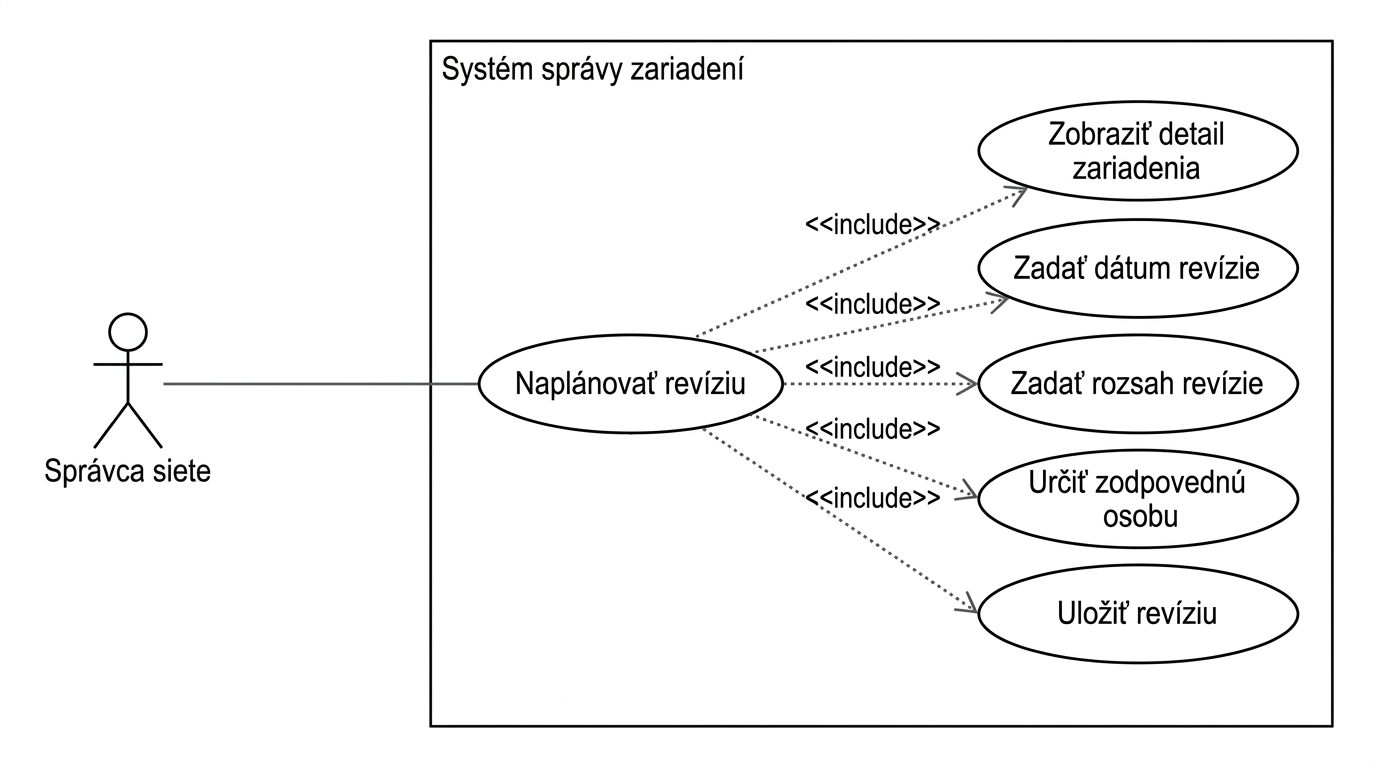
\includegraphics[width=\linewidth]{figures/1scenar.png}
    \caption{Use-case diagram pre scenár plánovania revízie.}
    \label{fig:1scenar}
\end{figure}

\clearpage

\subsection{Scenár 2 (Vykonanie revízie)}

\begin{itemize}
	\item \b{Aktér:} Revízny pracovník
	\item \b{Popis:} Zaznamenanie výsledku revízie
	\item \b{Predpoklady:} Revízia je naplánovaná, používateľ má oprávnenie
\end{itemize}

\subsubsection{Scenár:}

\begin{enumerate}
	\item používateľ otvorí zoznam revízií
	\item vyberie konkrétnu revíziu
	\item zadá výsledok (vyhovel / nevyhovel)
	\item doplní poznámku
	\item nahrá prílohy (protokol, foto)
	\item uloží záznam
\end{enumerate}

\subsubsection{Výsledok:}
\begin{itemize}
	\item revízia je uložená ako vykonaná
	\item aktualizuje sa stav zariadenia
\end{itemize}

\begin{figure}[htbp]
    \centering
    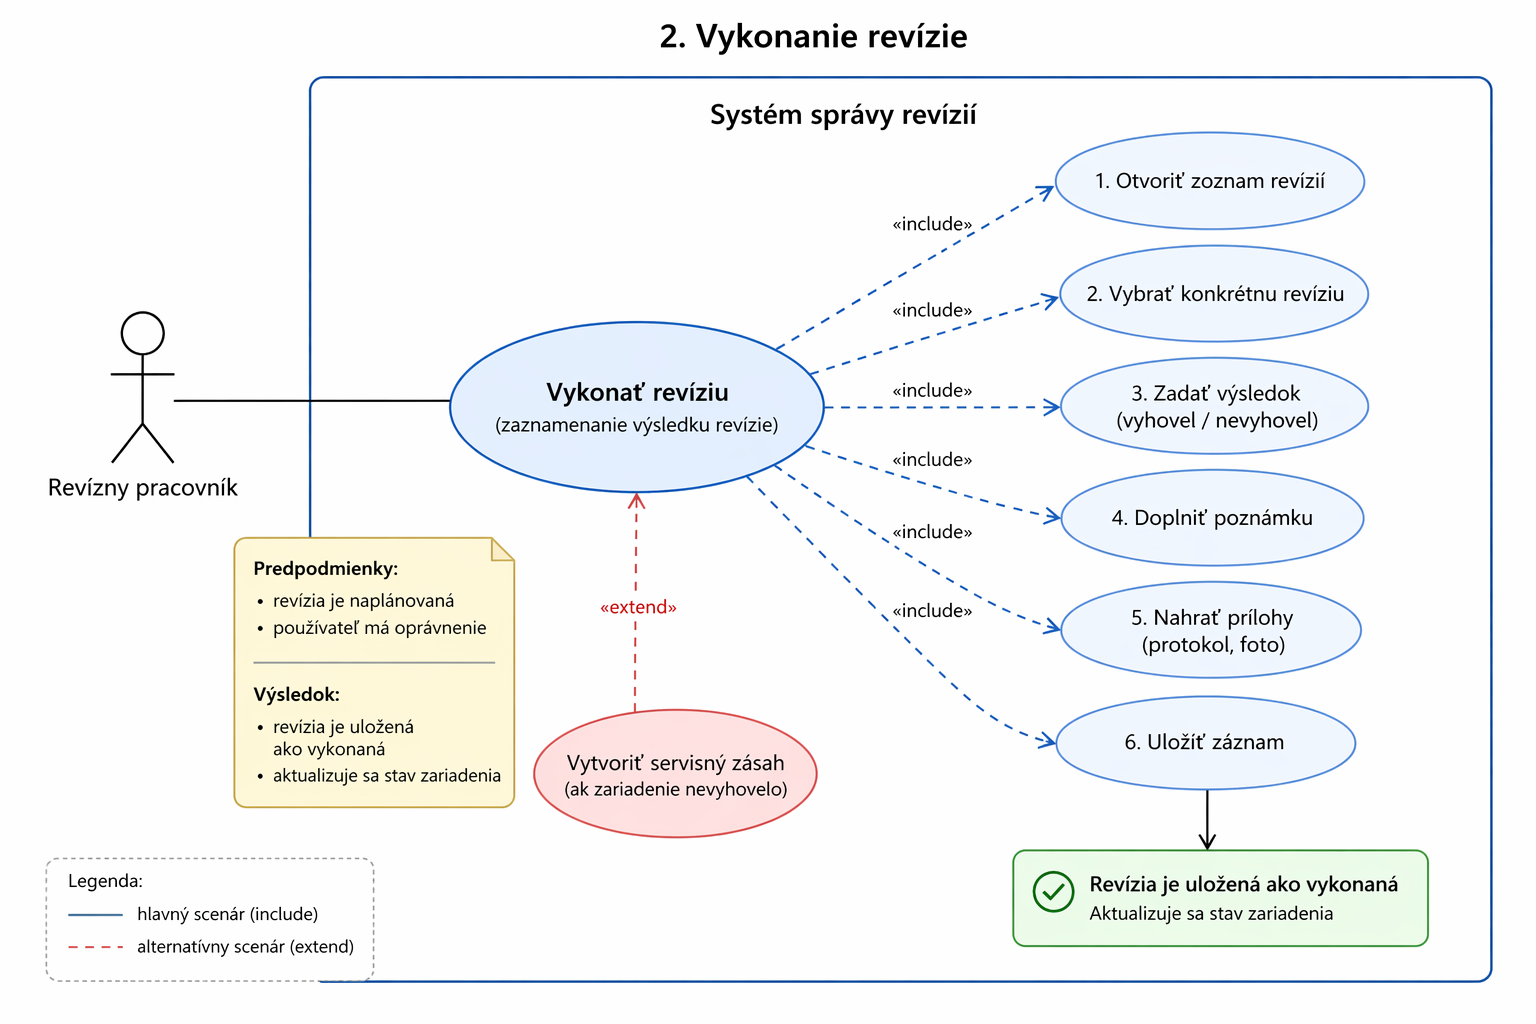
\includegraphics[width=\linewidth]{figures/2scenar.png}
    \caption{Use-case diagram pre scenár vykonanie revízie.}
    \label{fig:2scenar}
\end{figure}


\clearpage

\subsection{Scenár 3 (Servisný zásah)}

\begin{itemize}
	\item \b{Aktér:} Technik
	\item \b{Popis:} Vykonanie opravy alebo údržby
	\item \b{Predpoklady:} Existuje porucha alebo revízia s výsledkom „nevyhovel“
\end{itemize}

\subsubsection{Scenár:}

\begin{enumerate}
	\item používateľ otvorí servisný zásah
	\item nastaví stav „v riešení“
	\item vykoná opravu
	\item zapíše vykonané práce
	\item uvedie použitý materiál
	\item ukončí zásah
\end{enumerate}

\subsubsection{Výsledok:}
\begin{itemize}
	\item zásah je uložený
	\item zariadenie môže byť označené ako funkčné
\end{itemize}

\begin{figure}[htbp]
    \centering
    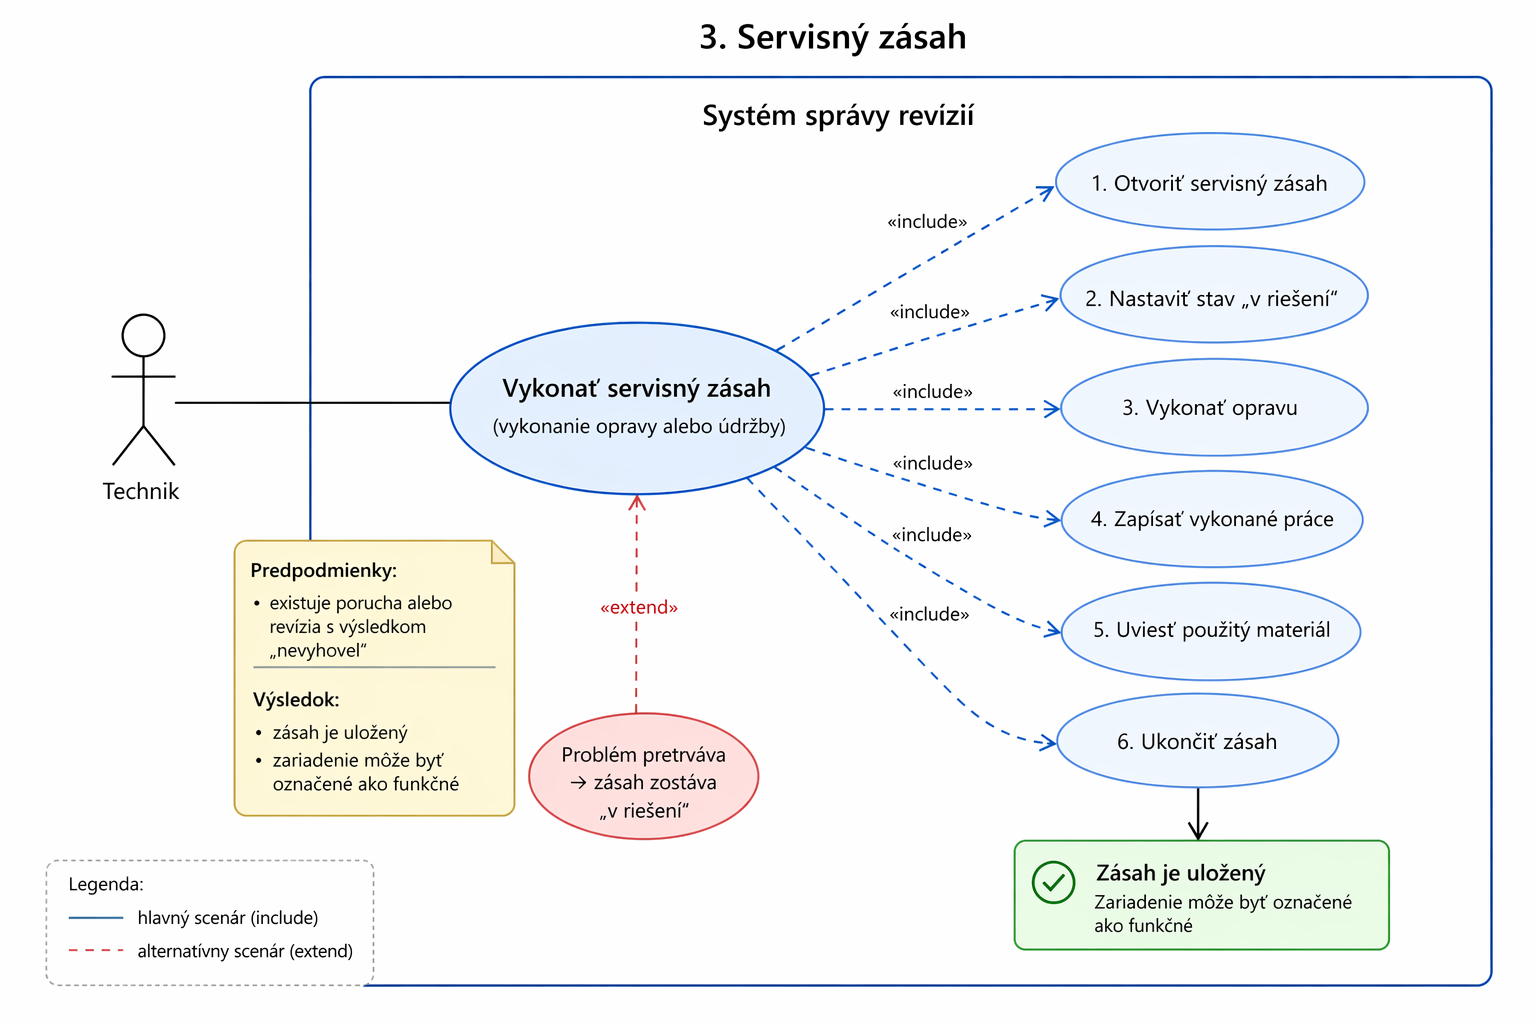
\includegraphics[width=\linewidth]{figures/3scenar.png}
    \caption{Use-case diagram pre scenár servisný zásah.}
    \label{fig:3scenar}
\end{figure}


\clearpage

\subsection{Scenár 4 (Generovanie reportu)}

\begin{itemize}
	\item \b{Aktér:} Manažér
	\item \b{Popis:} Vytvorenie reportu o revíziách alebo zásahoch
	\item \b{Predpoklady:} Existujú dáta v systéme
\end{itemize}

\subsubsection{Scenár:}

\begin{enumerate}
	\item používateľ otvorí sekciu reportov
	\item vyberie typ reportu
	\item nastaví filtre (dátum, zariadenie, stav)
	\item klikne „generovať“
	\item systém zobrazí výsledok
	\item používateľ exportuje report (PDF/CSV)
\end{enumerate}

\subsubsection{Výsledok:}
\begin{itemize}
	\item report je vygenerovaný a uložený
\end{itemize}

\begin{figure}[htbp]
    \centering
    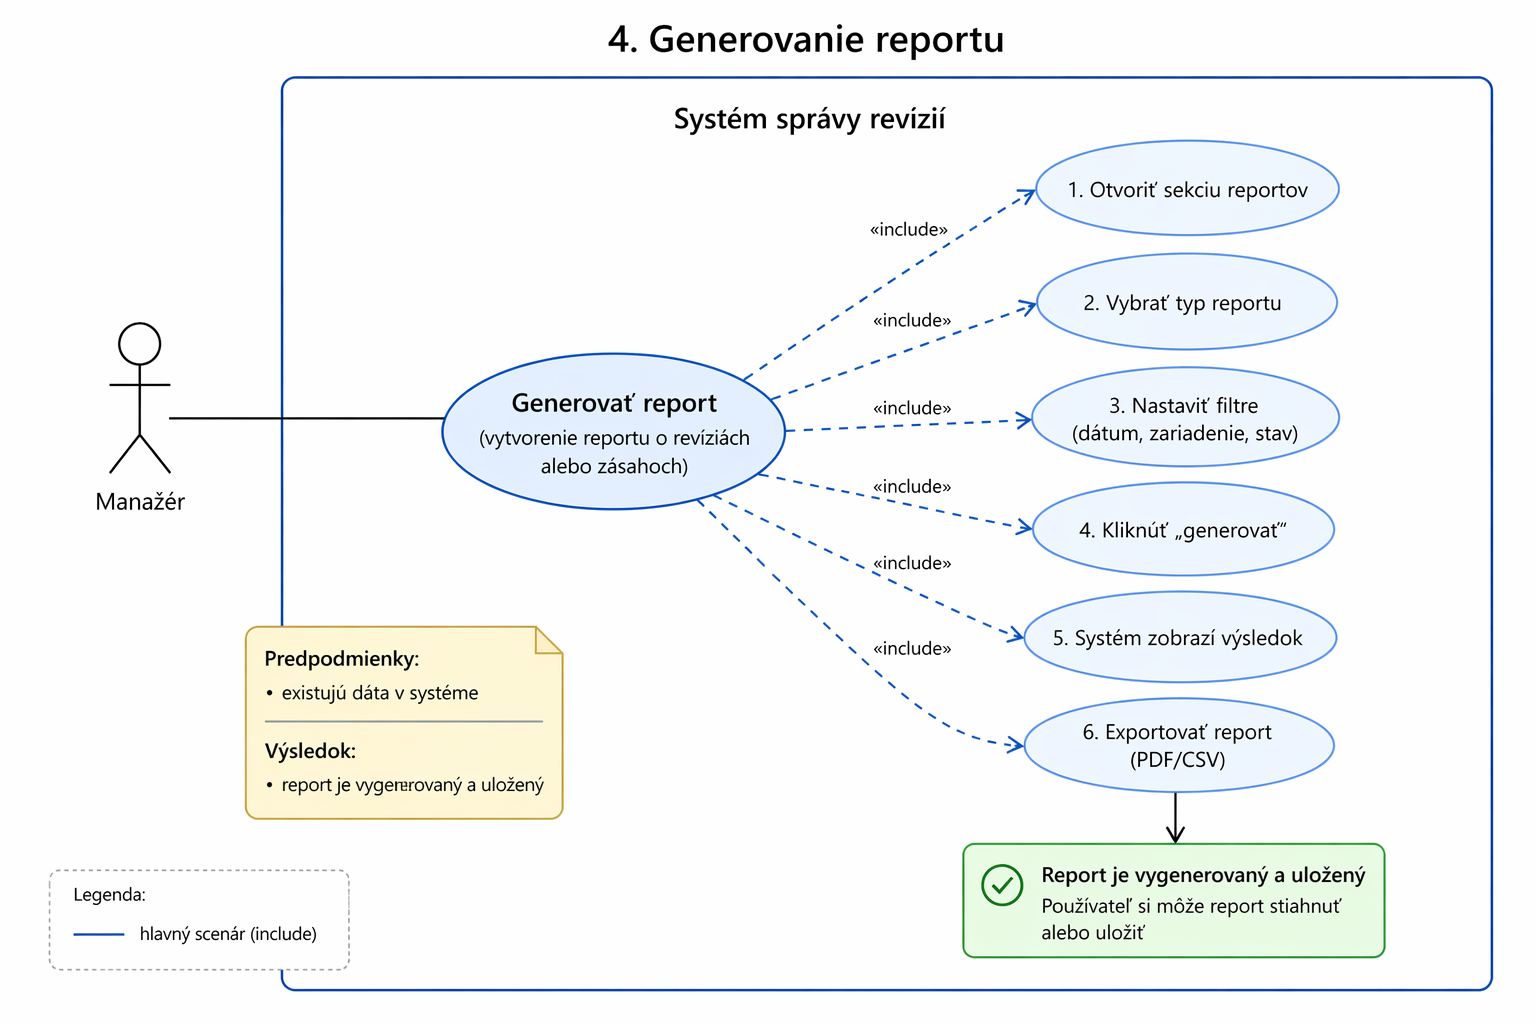
\includegraphics[width=\linewidth]{figures/4scenar.png}
    \caption{Use-case diagram pre scenár generovanie reportu.}
    \label{fig:4scenar}
\end{figure}

\clearpage

\subsection{Scenár 5 (Odoslanie notifikácie)}

\begin{itemize}
	\item \b{Aktér:} Systém (automatický proces)
	\item \b{Popis:} Informovanie používateľov o udalosti
	\item \b{Predpoklady:} Existuje naplánovaná alebo oneskorená revízia
\end{itemize}

\subsubsection{Scenár:}

\begin{enumerate}
	\item systém kontroluje termíny
	\item identifikuje blížiacu sa alebo oneskorenú revíziu
	\item vyberie príjemcov
	\item odošle notifikáciu (email / interná)
\end{enumerate}

\subsubsection{Výsledok:}
\begin{itemize}
	\item používateľ je informovaný
\end{itemize}

\begin{figure}[htbp]
    \centering
    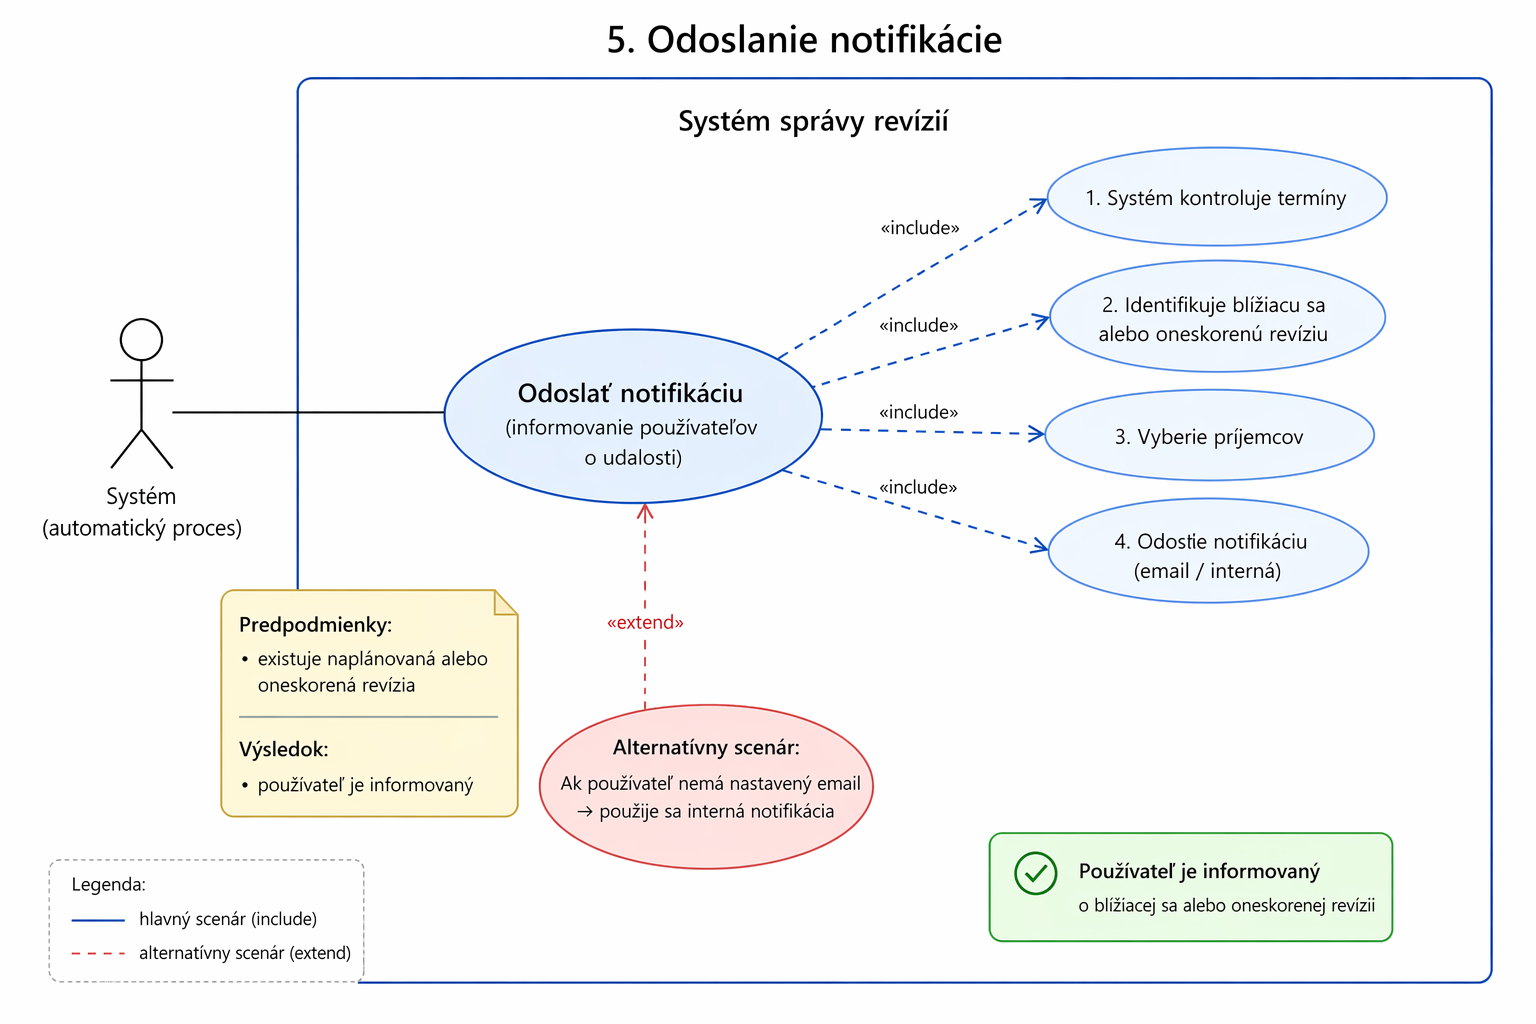
\includegraphics[width=\linewidth]{figures/5scenar.png}
    \caption{Use-case diagram pre scenár odoslanie notifikácie.}
    \label{fig:5scenar}
\end{figure}

\clearpage

\section{Overenie a príprava požiadaviek informačného systému}

\subsection{Stručné zhrnutie}

Nasledujúca doplňujúca časť vychádza z požiadaviek FR-01 až FR-12 a NFR-01 až NFR-08 uvedených v podkladových materiáloch. Z obsahového hľadiska tvoria tieto požiadavky kvalitný a prakticky použiteľný základ pre návrh systému. Obzvlášť dobre pripravené sú požiadavky na evidenciu zariadení, plánovanie a vykonanie revízií, export reportov a rolovo riadený prístup.

Pri ďalšom rozpracovaní sa oplatí jemne spresniť najmä konfiguračné hodnoty notifikácií, rozsah auditovaných operácií, výkonové hranice a parametre obnovy po zlyhaní. Regulačná opora tejto časti zostáva na existujúcich zdrojoch \cite{EUDWD2020,SKVyhlaska912023,UVZPitnaVodaMapy,NISTRBACGlossary,NIST80082R3}. Ako dopĺňajúce metodické zdroje pre vlastnosti požiadaviek, kvalitatívne kritériá, backlog a testovanie sú vhodné najmä \cite{ISO29148,ISO25010,ScrumGuide2020,ISTQBCTFL40}.

\subsection{Verifikácia požiadaviek}

Verifikácia v tejto práci znamená overenie, či je každá požiadavka formulovaná tak, aby bolo možné jednoznačne určiť spôsob testu, očakávaný výsledok a merateľné kritérium. Z metodického hľadiska je dôležité, aby požiadavka viedla k testovateľnému artefaktu a aby kvalitatívne požiadavky mali aspoň minimálne meradlá prijatia.

V posudzovanom dokumente sú funkčné požiadavky prevažne jednoznačné na úrovni toho, čo má systém vykonať, a preto poskytujú veľmi dobrý základ pre testovanie. Pri časti požiadaviek je užitočné doplniť presné hraničné hodnoty alebo prevádzkové limity, aby bolo možné dosiahnuť ešte vyššiu mieru konzistentného hodnotenia.

\footnotesize
\begin{longtable}{|p{1.8cm}|p{3.2cm}|p{4.3cm}|p{5.0cm}|}
\caption{Výsledky verifikácie vybraných požiadaviek}\label{tab:verification-requirements}\\
\hline
\textbf{ID} & \textbf{Spôsob verifikácie} & \textbf{Merateľné kritérium} & \textbf{Výsledok verifikácie} \\
\hline
\endfirsthead
\hline
\textbf{ID} & \textbf{Spôsob verifikácie} & \textbf{Merateľné kritérium} & \textbf{Výsledok verifikácie} \\
\hline
\endhead
FR-01 & funkčný test UI + kontrola dát & kartu zariadenia možno uložiť len po vyplnení minimálne: identifikátor, typ, umiestnenie, stav, dátum uvedenia do prevádzky & dobre verifikovateľná; povinné polia sú jasne špecifikované, odporúča sa doplniť formát a unikátnosť identifikátora \\
\hline
FR-04 & funkčný test plánovania revízie & revíziu možno uložiť len s termínom, rozsahom a pridelenou zodpovednou osobou; po uložení je viditeľná v harmonograme & veľmi dobre verifikovateľná; pre plnú jednoznačnosť možno doplniť pravidlo budúceho dátumu \\
\hline
FR-05 & funkčný test zápisu výsledku revízie & systém uloží výsledok revízie vrátane stavu, poznámky a príloh; záznam je spätne dohľadateľný v histórii zariadenia & dobre verifikovateľná; existencia záznamu je merateľná, pre vyššiu presnosť možno doplniť povinnosť a typ príloh \\
\hline
FR-09 & integračný test plánovača + notifikačného kanála & pred termínom revízie sa odošle notifikácia príslušnému používateľovi; v logu je čas, príjemca, kanál a výsledok odoslania & dobre verifikovateľná; požiadavka je jasná, odporúča sa doplniť predstih N dní \\
\hline
FR-12 & funkčný test reportingu a exportu & pre zvolený report vzniknú exporty aspoň vo formáte PDF a CSV; export obsahuje rovnakú dátovú množinu podľa zadaného filtra & veľmi dobre verifikovateľná; pre prevádzkovú istotu možno doplniť výkonový limit a maximálny objem dát \\
\hline
NFR-01 & bezpečnostný test prihlásenia a oprávnení & neprihlásený používateľ sa k dátam nedostane; prihlásený používateľ vidí len artefakty povolené rolou & veľmi dobre verifikovateľná; pre úplnú konzistentnosť sa odporúča zafixovať testovaciu maticu rolí a oprávnení \\
\hline
NFR-02 & bezpečnostný test komunikácie & celý systém je dostupný cez HTTPS; nezabezpečený prístup je blokovaný alebo presmerovaný; prihlasovacie údaje sa neprenášajú po HTTP & veľmi dobre verifikovateľná; pre úplnú špecifikáciu možno doplniť minimálnu verziu TLS a detaily certifikátovej politiky \\
\hline
NFR-03 & auditný test kritických operácií & pri vytvorení, úprave, zmene stavu alebo exporte vznikne auditný záznam aspoň s používateľom, časom, objektom a výsledkom operácie & dobre verifikovateľná; princíp je jasný, odporúča sa doplniť úplný zoznam dôležitých operácií \\
\hline
NFR-06 & test zálohovania a obnovy & vytvorí sa pravidelná záloha a systém je možné obnoviť do konzistentného stavu bez straty štruktúry dát & dobre verifikovateľná; pre ešte lepšiu merateľnosť sa odporúča doplniť periodicitu záloh, RPO a RTO \\
\hline
\end{longtable}
\normalsize

Z pohľadu ďalšieho spresnenia majú najvyššiu prioritu FR-09, NFR-03 a NFR-06. Doplnenie týchto troch oblastí prinesie rýchly nárast jednoznačnosti a ešte hladší priebeh akceptačného testovania.

\subsection{Validácia požiadaviek}

Validácia odpovedá na otázku, či požiadavky stále zodpovedajú legislatíve, prevádzke a potrebám používateľských rolí. V čase spracovania tejto kapitoly zostáva regulačný základ platný: smernica 2020/2184 je účinná, členské štáty mali transponovať relevantné ustanovenia do 12. januára 2023, časť prechodných povinností dobehla 12. januára 2026 a rámec bol ďalej dopĺňaný delegovanými aktmi EÚ \cite{EUDWD2020,EUDWDDelegated2024}. Slovenská vyhláška 91/2023 upravuje ukazovatele kvality pitnej vody, programy monitorovania a manažment rizík a je účinná od 1. apríla 2023 \cite{SKVyhlaska912023}.

Prevádzková validita je rovnako zachovaná. Oprávnenosť požiadaviek na evidenciu zariadení, revízií, servisných zásahov, reportov a auditnej stopy podporuje aj priebežný monitoring pitnej vody v slovenskej praxi \cite{UVZPitnaVodaMapy}. Pre používateľské roly ADM, NET, TECH, REV a MAN preto požiadavky na register, revízie, zásahy, notifikácie a reporty ostávajú vecne platné; meniť sa budú skôr ich detaily, nie samotná existencia.

\footnotesize
\begin{longtable}{|p{3.3cm}|p{4.2cm}|p{3.8cm}|p{3.2cm}|}
\caption{Validita požiadaviek a spúšťače ich revízie}\label{tab:requirements-validity}\\
\hline
\textbf{Oblasť požiadaviek} & \textbf{Dôvod platnosti} & \textbf{Predpokladaná platnosť} & \textbf{Spúšťač revízie požiadavky} \\
\hline
\endfirsthead
\hline
\textbf{Oblasť požiadaviek} & \textbf{Dôvod platnosti} & \textbf{Predpokladaná platnosť} & \textbf{Spúšťač revízie požiadavky} \\
\hline
\endhead
Legislatívna zhoda, monitoring a manažment rizík & vyplýva z požiadaviek na kvalitu pitnej vody, monitoring a riadenie rizík & do ďalšej novely právnych predpisov; formálne kontrolovať minimálne raz ročne & novela smernice, delegovaný akt EÚ, novela vyhlášky, zmena požiadaviek regulátora \\
\hline
Evidencia zariadení a väzieb & register je základom pre revízie, servis, reporty aj audit & dlhodobá, spravidla 2--3 roky bez zmeny jadra modelu & zmena dátového modelu, nové typy zariadení, integrácia GIS/CMMS \\
\hline
Revízie a servisné zásahy & ide o jadro prevádzky a preukázateľnosť plnenia povinností & dlhodobá; obsah kontrolovať pri každej ročnej revízii procesov & zmena periodicity kontrol, zmena servisného procesu, outsourcing alebo nové protokoly \\
\hline
Bezpečnosť, roly a RBAC & potreba minimálnych oprávnení a oddelenia zodpovedností ostáva stabilná & platná priebežne; minimálne ročný review & organizačná zmena, nové roly, externý dodávateľ, SSO/IdP integrácia, bezpečnostný incident \\
\hline
Notifikácie a eskalácie & znižujú riziko zmeškaných termínov a oneskorených zásahov & funkčne dlhodobá, konfiguračne 6--12 mesiacov & zmena interných lehôt, veľa falošných upozornení, nový komunikačný kanál \\
\hline
Reporty, export a audit & potreba manažérskeho dohľadu a kontroly súladu ostáva trvalá & 12--24 mesiacov pre formát a rozsah; funkčne dlhodobá & nový formát pre regulátora, požiadavka API exportu, nové metadáta alebo archivácia \\
\hline
Zálohovanie a obnova & nevyhnutné pre kontinuitu prevádzky & platná priebežne; parametre preskúmať aspoň polročne & zmena infraštruktúry, neúspešný disaster-recovery test, nové RPO/RTO \\
\hline
\end{longtable}
\normalsize

\subsection{Príprava pre návrh a implementáciu}

Prevod požiadaviek do vývojového backlogu má zmysel postaviť na menších, transparentných položkách, ktoré sú dostatočne presné na výber do sprintu a majú spoločné akceptačné kritériá. Takýto prístup znižuje riziko odchýlky implementácie od pôvodnej požiadavky a zároveň zlepšuje prevzatie výsledkov.

\subsubsection*{Epic: Register zariadení}
\textbf{Väzba:} FR-01, FR-02, FR-03, NFR-03.\\
\textbf{User story:} Ako správca siete chcem založiť a upravovať kartu zariadenia, aby som mal jednotný register použiteľný pre revízie a servis.
\begin{itemize}
\item systém neuloží kartu bez minimálnych povinných údajov,
\item po uložení je zariadenie vyhľadateľné podľa typu, lokality, stavu a zodpovednej osoby,
\item každá úprava vytvorí históriu zmien,
\item zmena zariadenia vytvorí auditný záznam.
\end{itemize}

\subsubsection*{Epic: Revízie}
\textbf{Väzba:} FR-04, FR-05, FR-06, NFR-01, NFR-03.\\
\textbf{User story:} Ako revízny pracovník chcem mať naplánovanú revíziu s termínom a rozsahom, aby som vedel vykonať kontrolu v správnom čase a s úplným záznamom.
\begin{itemize}
\item revíziu možno vytvoriť len s termínom, rozsahom a zodpovednou osobou,
\item po vykonaní možno uložiť výsledok, poznámku a prílohy,
\item každá revízia sa zobrazí v histórii konkrétneho zariadenia v časovom poradí,
\item prístup k revízii rešpektuje rolu používateľa.
\end{itemize}

\subsubsection*{Epic: Servisné zásahy}
\textbf{Väzba:} FR-07, FR-08, NFR-03.\\
\textbf{User story:} Ako technik údržby chcem založiť a priebežne dopĺňať servisný zásah, aby bolo možné spätne preukázať vykonané práce, použitý materiál a zodpovednosť.
\begin{itemize}
\item zásah možno založiť z podnetu, z poruchy alebo z nevyhovujúcej revízie,
\item zásah je naviazaný na konkrétne zariadenie a podľa potreby aj na revíziu,
\item pri zásahu je možné evidovať práce, materiál a zodpovednú osobu,
\item uzavretie zásahu sa zapíše do auditu.
\end{itemize}

\subsubsection*{Epic: Notifikácie}
\textbf{Väzba:} FR-09, FR-10, NFR-01, NFR-02, NFR-03.\\
\textbf{User story:} Ako správca siete chcem dostávať upozornenia pred termínom a po termíne revízie, aby som vedel včas reagovať na riziko omeškania.
\begin{itemize}
\item systém odošle upozornenie pred termínom podľa konfigurovanej hodnoty N,
\item po prekročení termínu sa vytvorí eskalačné upozornenie,
\item pri odoslaní sa eviduje čas, kanál, príjemca a výsledok,
\item notifikáciu nemožno zobraziť používateľovi bez príslušného oprávnenia.
\end{itemize}

\subsubsection*{Epic: Reporty a audit}
\textbf{Väzba:} FR-11, FR-12, NFR-03, NFR-07.\\
\textbf{User story:} Ako manažér chcem generovať report revízií a exportovať ho do PDF a CSV, aby som mal podklady pre riadenie, kontrolu a audit.
\begin{itemize}
\item používateľ zvolí obdobie a typ reportu,
\item systém vygeneruje konzistentný výstup v PDF aj CSV,
\item report je spätne dohľadateľný podľa typu a dátumu,
\item generovanie a export reportu vytvoria auditný záznam.
\end{itemize}

Ak sa backlog bude ďalej spresňovať, odporúča sa doplniť pre každý epic explicitnú Definition of Done, najmä pre bezpečnostné, auditné a exportné časti.

\subsection{Príprava pre testovanie}

Testovacie prípady majú byť naviazané priamo na FR/NFR a majú pokrývať nielen funkčnosť, ale aj rozhrania, bezpečnosť a prevzatie systému používateľom. V metodickej rovine je vhodné odlíšiť testovacie úrovne a typy testov \cite{ISTQBCTFL40}.

\begingroup
\footnotesize
\setlength{\tabcolsep}{2pt}
\begin{longtable}{|p{1.2cm}|p{1.8cm}|p{2.0cm}|p{3.2cm}|p{3.0cm}|p{1.3cm}|}
\caption{Návrh testovacích prípadov nad FR/NFR požiadavkami}\label{tab:test-cases-requirements}\\
\hline
\textbf{ID testu} & \textbf{Väzba} & \textbf{Predpoklady} & \textbf{Testovacie kroky} & \textbf{Očakávaný výsledok} & \textbf{Typ} \\
\hline
\endfirsthead
\hline
\textbf{ID testu} & \textbf{Väzba} & \textbf{Predpoklady} & \textbf{Testovacie kroky} & \textbf{Očakávaný výsledok} & \textbf{Typ} \\
\hline
\endhead
TC-F-01 & FR-01 & používateľ NET je prihlásený & otvorí formulár zariadenia, vyplní minimálne polia, uloží záznam & systém uloží kartu zariadenia a zobrazí ju v registri & funkčný \\
\hline
TC-F-02 & FR-04 & existuje zariadenie a používateľ NET & vytvorí revíziu, zadá termín, rozsah a zodpovednú osobu, uloží & revízia je uložená v harmonograme s väzbou na zariadenie & funkčný \\
\hline
TC-F-03 & FR-05 & existuje naplánovaná revízia a používateľ REV & otvorí revíziu, zapíše výsledok, poznámku a priloží súbor & revízia sa uloží ako vykonaná a je zobrazená v histórii zariadenia & funkčný \\
\hline
TC-I-01 & FR-09 & existuje revízia pred termínom; nastavený notifikačný kanál & spustí sa plánovač alebo dávka, systém vyhodnotí blížiaci sa termín & príslušný príjemca dostane notifikáciu a v logu je záznam o odoslaní & integračný \\
\hline
TC-I-02 & FR-10 & existuje oneskorená revízia alebo servisný zásah & systém vyhodnotí stav po termíne & revízia alebo zásah sú označené ako po termíne a vznikne eskalačné upozornenie & integračný \\
\hline
TC-F-04 & FR-12 & existujú dáta pre report; používateľ MAN & zvolí obdobie, vygeneruje report, exportuje PDF a CSV & oba exporty sú vytvorené a obsahovo zodpovedajú zvolenému filtru & funkčný \\
\hline
TC-S-01 & NFR-01 & existujú účty REV a MAN s rozdielnymi rolami & REV sa pokúsi otvoriť objekt mimo svojich oprávnení; MAN otvorí povolený report & nepovolený prístup je zamietnutý, povolený je úspešný & bezpečnostný \\
\hline
TC-S-02 & NFR-02 & testovacie prostredie je dostupné zvonka & skúsi otvoriť systém cez HTTP a následne cez HTTPS & prístup je vynútený cez HTTPS; citlivé dáta sa neprenesú po HTTP & bezpečnostný \\
\hline
TC-S-03 & NFR-03 & audit je zapnutý & používateľ vytvorí zariadenie, upraví revíziu a vygeneruje report & v audite vzniknú záznamy s aspoň používateľom, časom, objektom a typom operácie & bezpečnostný \\
\hline
TC-R-01 & NFR-06 & existuje posledná záloha testovacej databázy & vyvolá sa obnova zo zálohy do čistého prostredia & systém sa obnoví do konzistentného stavu; cieľový čas obnovy sa následne potvrdí v prevádzkových parametroch & obnova \\
\hline
TC-A-01 & FR-11, FR-12, NFR-01, NFR-03 & používateľ MAN alebo AUD má príslušné práva & zvolí obdobie, vygeneruje report, exportuje ho a odovzdá ako podklad pre kontrolu & používateľ vie samostatne získať čitateľný a dohľadateľný výstup bez zásahu administrátora & akceptačný \\
\hline
\end{longtable}
\normalsize
\endgroup

Za minimálnu sadu pred implementáciou do produkcie možno považovať testy TC-F-01 až TC-F-04, TC-I-01, TC-S-01, TC-S-03 a TC-A-01. Pred začiatkom testovania je vhodné doplniť najmä tieto hodnoty: konfigurovaný predstih notifikácie N, zoznam kritických auditovaných operácií, pravidelnosť záloh, prípustnú stratu dát pri obnove a očakávaný čas obnovy systému.